% Appendix: calibration pilot, diagnosis and revisions (2026-11-18).
% Standalone: compiles with the apa7 class (manuscript mode) + natbib; the reference list is written by hand
% (thebibliography, APA 7 format), so only pdfLaTeX is needed, no biber/bibtex run.
%   latexmk -pdf appendix_calibration.tex
% Figures are in ./figures/ (PNG, 200 dpi); they were drawn from the pilot data with the scripts
% kept in the session scratchpad (fig*.py) and can be regenerated from data/*_simple_calib_trials.csv.
% Not compiled in the development container (no TeX installation there).
\documentclass[man,12pt,floatsintext,natbib]{apa7}
\usepackage[american]{babel}
\usepackage{csquotes}
\usepackage{graphicx}
\graphicspath{{figures/}}
\usepackage{booktabs}
\usepackage{amsmath}
\usepackage{siunitx}

\title{Appendix: Calibration Pilot, Diagnosis, and Revisions of the Adaptive SFT Procedure}
\shorttitle{Calibration pilot}
\authorsnames{}
\authorsaffiliations{}

\begin{document}
\appendix

\section{Overview}

This appendix documents a calibration failure observed in the third pilot session of the audiovisual working-memory SFT task (participant EN01, 18 November 2026), the analyses that located its cause, and the revisions to the calibration procedure that followed. The calibration estimates, for each participant and each dimension (colour difference in $\Delta E_{00}$; consonant distinctiveness in $d'$ units), the two stimulus values that are used as the high- (H) and low-salience (L) levels in the double-factorial design \citep{houpt2014}. The failure was that both colour values were returned as $\Delta E = 2$, the smallest presentable level, so that the colour manipulation was absent from the 576 main-task trials that followed. Section~\ref{sec:data} describes the data; Section~\ref{sec:mechanism} traces the value~2 to its origin; Sections~\ref{sec:criterion}--\ref{sec:estimator} give the three model-side revisions (a response criterion, a saturating link function, and a median point estimator); Section~\ref{sec:levels} gives the design-side revision (stimulus levels); Section~\ref{sec:sound} reports the corresponding check of the auditory dimension and the resulting decision to present the consonants in speech-shaped noise. All figures were produced from the pilot data; each figure's note states the quantities plotted.

\section{Calibration Data}\label{sec:data}

Each calibration block presents the full working-memory trial (two colours and two consonants studied, one probe) with only one dimension varied. Six stimulus levels are presented five times each with the probe differing from the studied item on the calibrated dimension (30 \enquote{different} trials, the other dimension held at the studied value), plus match trials in which the probe is identical (10 \enquote{same} trials), with trial-by-trial feedback withheld. Responses are \emph{same} / \emph{different}. The colour levels at the time of the pilot were $\Delta E \in \{2, 6, 12, 25, 50, 90\}$; the sound levels were $d' \in \{0.4, 0.9, 1.5, 2.3, 3.3, 4.5\}$ on the consonant-pair scale derived from \citet{millernicely1955} (see the main text). The model fitted after each block is the lognormal race model of \citet{houpt2014} (their \texttt{lnrm2}), in which a correct and an incorrect accumulator have log-normal finishing times with means $\mu - d(x)$ and $\mu + d(x)$, common standard deviation $\sigma$, and a non-decision time $\psi$; the drift advantage $d(x)$ was a quadratic function of stimulus intensity $x$, $d(x) = \alpha x + \alpha_2 x^2$, with $x$ expressed as $\Delta E / 10$ for colour and $d'$ for sound. H and L were obtained by inverting $2\,d(x)$ at the drift-separation targets 8.0 and 1.3 on every posterior draw and averaging the solutions, as in the authors' R code.

Three pilot participants contributed: yycy (3 November; non-native listener; sound scale of an earlier version), yyc1110 (10 November), and EN01 (18 November). Table~\ref{tab:colour} gives the colour accuracies. All three were at the false-alarm floor at $\Delta E \le 12$ and at ceiling from 50 upward; their proportions of \emph{different} responses on the 10 same trials were .10 (EN01) and similar for the others.

\begin{table}[htbp]
\caption{Proportion of \emph{Different} Responses on Colour Calibration Trials, by Level and Participant}
\label{tab:colour}
\begin{tabular}{lcccccc}
\toprule
 & \multicolumn{6}{c}{$\Delta E_{00}$} \\
\cmidrule(lr){2-7}
Participant & 2 & 6 & 12 & 25 & 50 & 90 \\
\midrule
yycy    & .00 & .20 & .60 & 1.00 & 1.00 & 1.00 \\
yyc1110 & .20 & .20 & .00 & 1.00 & 1.00 & .80 \\
EN01    & .20 & .20 & .00 & .60  & 1.00 & .80 \\
\bottomrule
\end{tabular}
\note{Five trials per level per participant; \emph{different} is the correct response on these trials.}
\end{table}

\section{Origin of the Value 2}\label{sec:mechanism}

The value 2 was not a fitted quantity. It is $\min(\text{levels})$, produced by two range-handling rules in the experiment script after the inversion returned a negative number for H. The negative number arose in three steps, each visible in Figures~\ref{fig:floor}--\ref{fig:Lroots}, which refit the model exactly as the script had run it (same link, same priors, 4 chains $\times$ 1{,}000 draws).

\paragraph{The model's floor does not match the task's floor.} The race model with $d(0) = 0$ predicts that at zero stimulus difference the two accumulators are equally fast, i.e.\ a \SI{50}{\percent} probability of the \emph{different} response. That prediction is appropriate for a two-alternative task with symmetric alternatives, as in \citet{houpt2014}. In a same/different task the correct response at zero difference is \emph{same}, and observers give it almost always: EN01's proportion of \emph{different} responses was .10 on same trials and .00--.20 at $\Delta E \le 12$ (Figure~\ref{fig:floor}).

\paragraph{The slope becomes sign-ambiguous.} To reproduce a \SI{10}{\percent} floor the symmetric model must make $d(x)$ negative at small $x$, while the ceiling at $\Delta E \ge 50$ requires $d(x)$ positive. The posterior of $\alpha$ therefore straddled zero, $P(\alpha < 0) = .50$ (Figure~\ref{fig:alpha}), and the curvature $\alpha_2$ was centred on zero.

\paragraph{A few draws return enormous negative roots.} The inversion $x = \left(-\alpha/\alpha_2 - \sqrt{(\alpha/\alpha_2)^2 + 2\,t/\alpha_2}\right)/2$ was evaluated on the draws with $\alpha_2 < 0$. For the H target only 30 of 1{,}314 such draws had a real root; 28 of them, with $\alpha > 0$, gave 225--1{,}348 $\Delta E$, and two, with $\alpha < 0$ and $\alpha_2$ within $10^{-4}$ of zero, gave $-17{,}000$ and $-27{,}000$ $\Delta E$ (Figure~\ref{fig:Hroots}). The arithmetic mean over the 30 was $-994$; the median was 431. The L target had 507 solvable draws, four of them negative, mean $-50$, median 50 (Figure~\ref{fig:Lroots}).

\paragraph{Range handling converted one failure into two.} The script clipped H into the presentable range $[2, 90]$, which maps any negative value to 2, and then applied the rule \enquote{if $L \ge H$, set $L$ to the lowest level}, written on the assumption that an inverted order means L is wrong. Here H was wrong, and the rule reduced a usable L to 2 as well. The same session's auditory calibration was unaffected ($H = 4.5$ after clipping, $L = 0.93$).

\begin{figure}[htbp]
\caption{Colour Calibration Data of EN01 Against the Floor Assumed by the Symmetric Race Model}
\label{fig:floor}
\centering
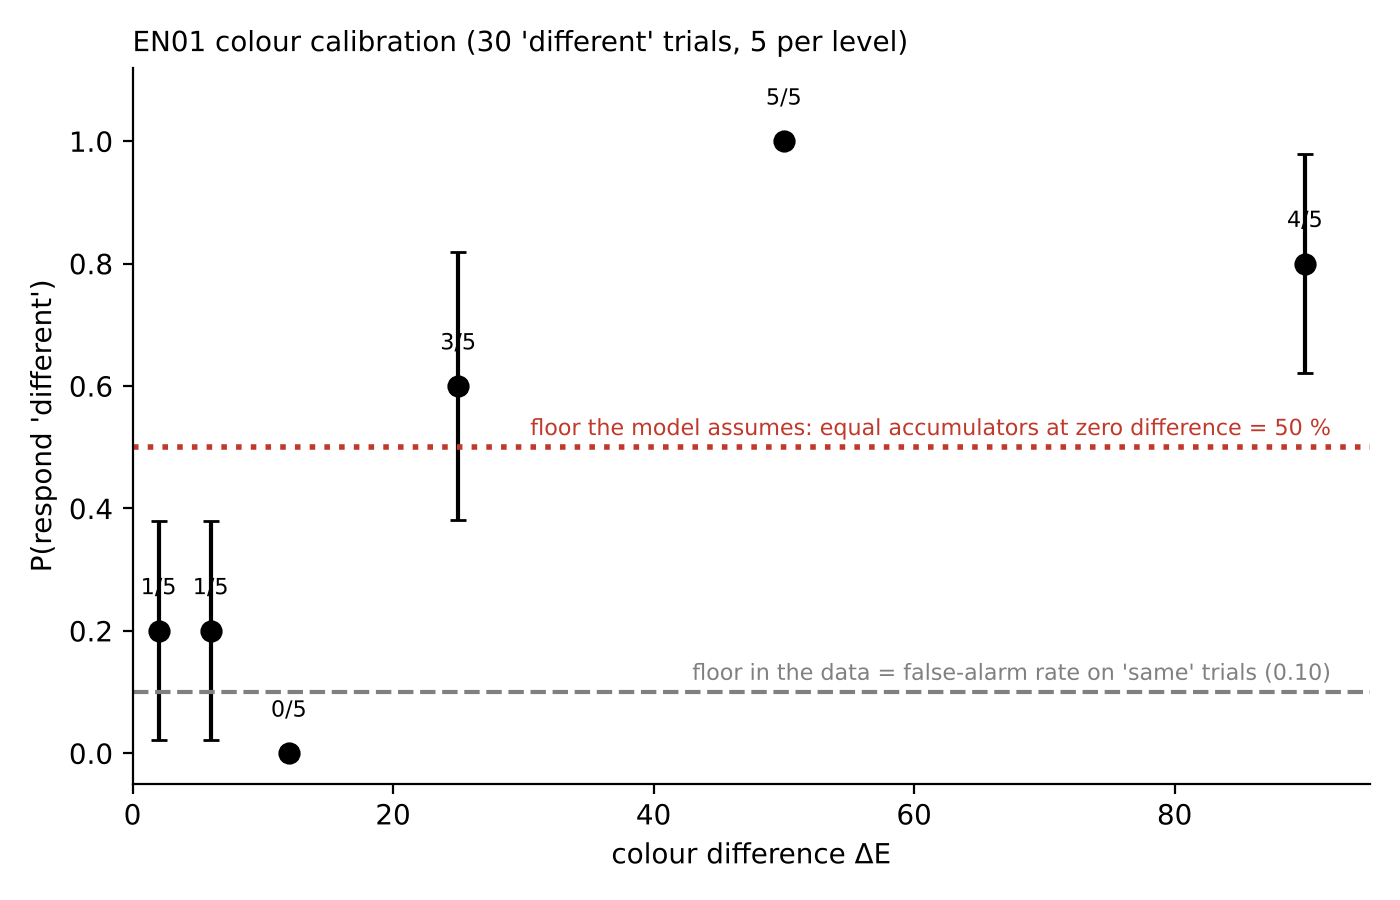
\includegraphics[width=\linewidth]{fig1_data_vs_model_floor}
\note{Points are the proportion of \emph{different} responses at each level (5 trials each; bars are binomial standard errors). The dashed line is the false-alarm rate on same trials (.10), the task's empirical floor; the dotted line is the \SI{50}{\percent} floor implied by $d(0) = 0$.}
\end{figure}

\begin{figure}[htbp]
\caption{Posterior Distribution of the Slope $\alpha$ Under the Symmetric Model}
\label{fig:alpha}
\centering
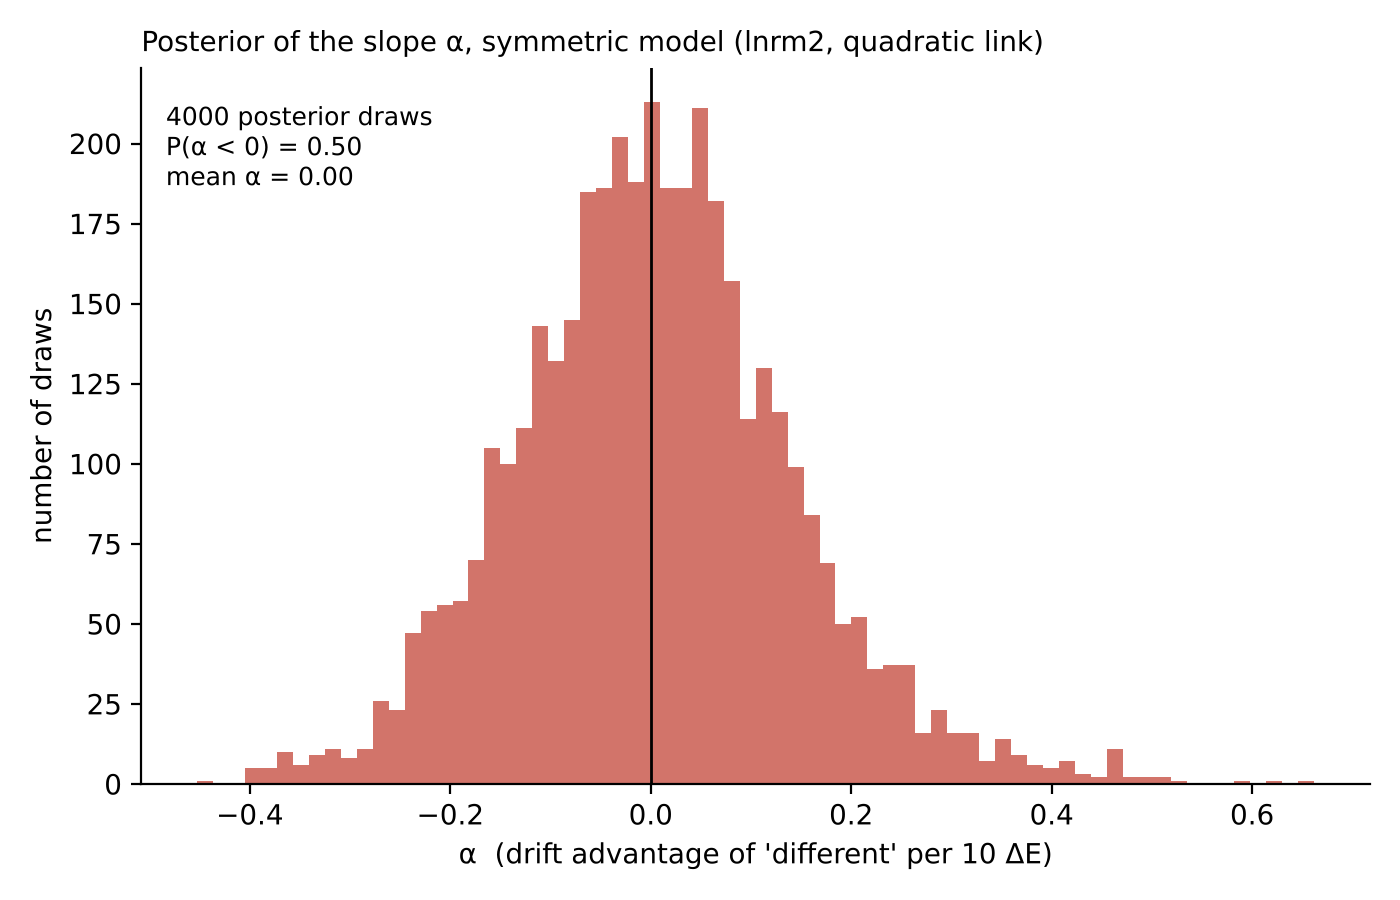
\includegraphics[width=\linewidth]{fig2_alpha_posterior}
\note{Quadratic link, no criterion; 4{,}000 draws. $P(\alpha < 0) = .50$.}
\end{figure}

\begin{figure}[htbp]
\caption{Inverted H Across the Solvable Posterior Draws}
\label{fig:Hroots}
\centering
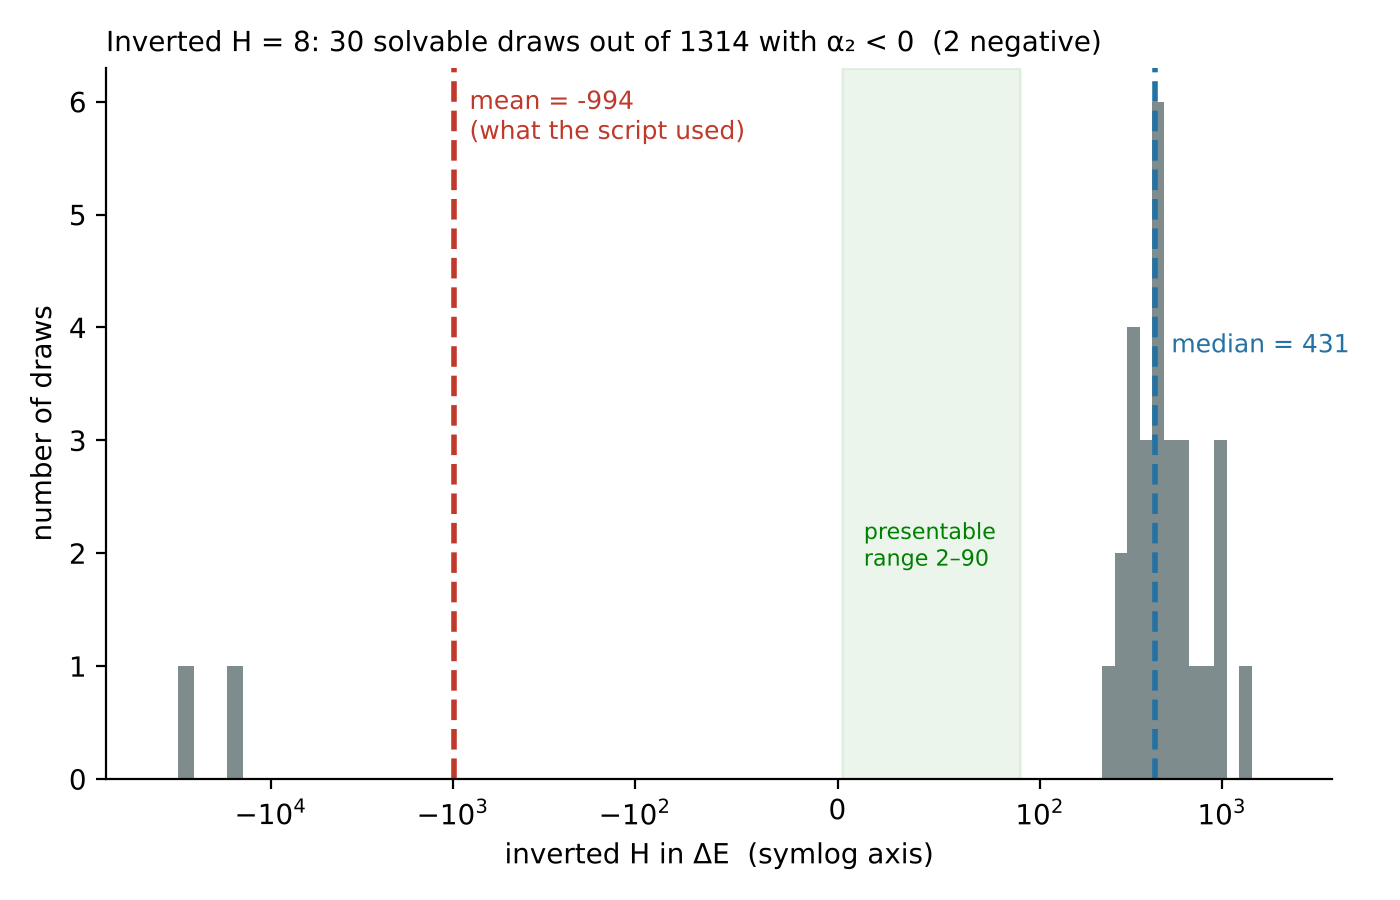
\includegraphics[width=\linewidth]{fig3_H_root_distribution}
\note{Symmetric-log abscissa. Of 1{,}314 draws with $\alpha_2 < 0$, 30 had a real root for the H target; two were negative. Red: mean ($-994$), the summary used by the script; blue: median (431). The green band is the presentable range.}
\end{figure}

\begin{figure}[htbp]
\caption{Inverted L Across the Solvable Posterior Draws}
\label{fig:Lroots}
\centering
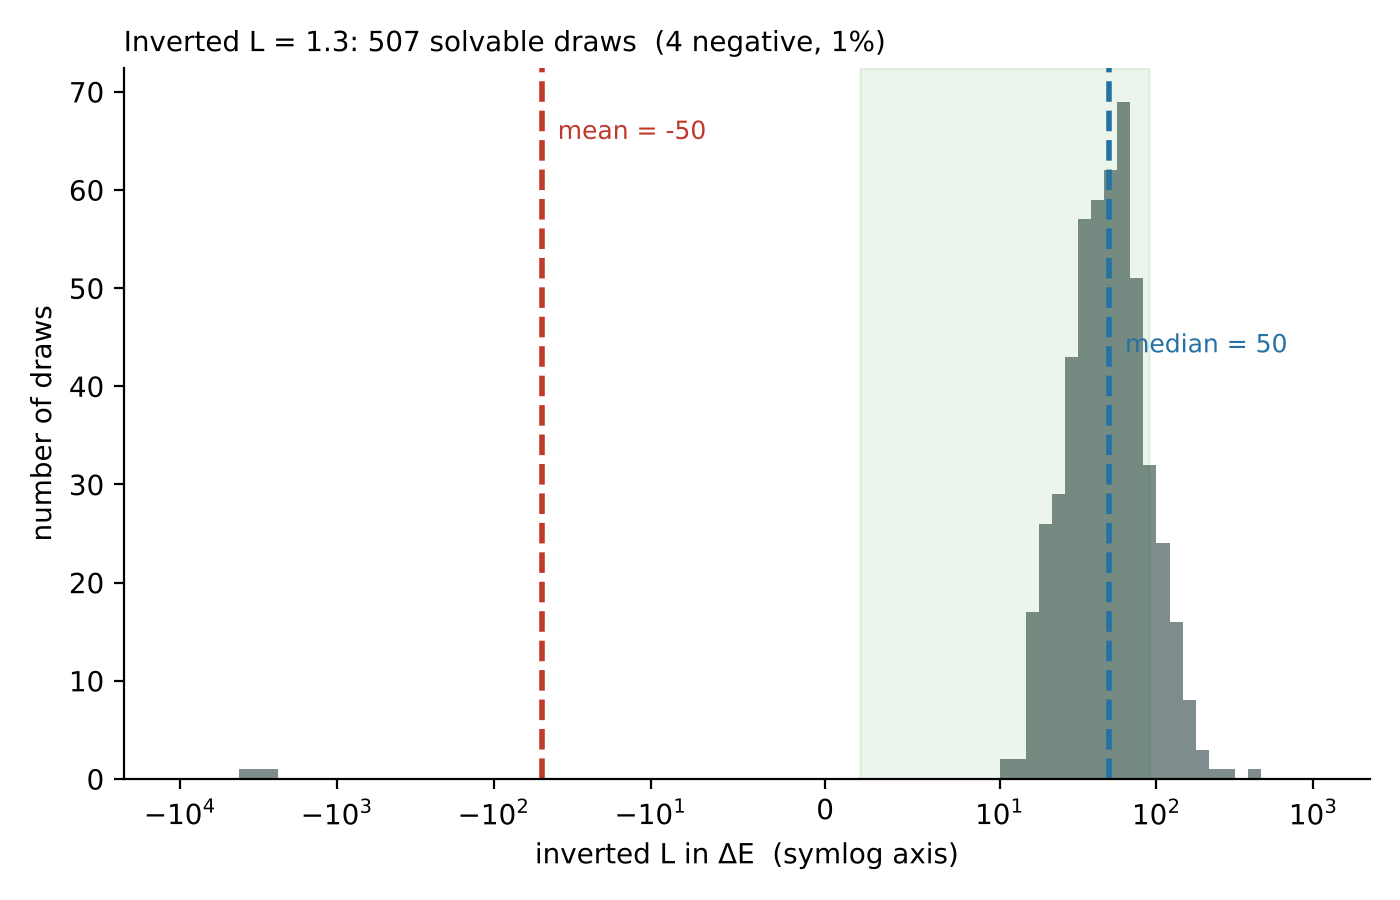
\includegraphics[width=\linewidth]{fig4_L_root_distribution}
\note{As Figure~\ref{fig:Hroots}, for the L target: 507 solvable draws, four negative, mean $-50$, median 50.}
\end{figure}

\section{Revision 1: A Response Criterion}\label{sec:criterion}

The structural mismatch is removed by one additional parameter, an intercept $b_0$ in the drift advantage, $d_{\text{eff}}(x) = b_0 + d(x)$, with $b_0 \sim \mathcal{N}(0, 2)$. With $b_0 < 0$ the \emph{same} accumulator starts ahead, and the predicted proportion of \emph{different} responses at zero difference equals the observer's false-alarm rate rather than .5. $b_0$ is the same/different criterion of signal detection theory \citep{macmillan2005}; it is a property of every observer in this task, not a peculiarity of the pilot. Figure~\ref{fig:tasks} shows the two task structures under the same race model; Figures~\ref{fig:alphab0} and \ref{fig:predb0} show the effect on EN01's data. With $b_0$ the same 30 trials gave $b_0 = -1.35$ (\SI{90}{\percent} interval $[-2.09, -0.62]$), $\alpha = 0.72$ with $P(\alpha < 0) = .00$, and $\alpha_2 = -0.057$ with $P(\alpha_2 < 0) = .99$. The predicted proportions of \emph{different} responses at $\Delta E = 2, 12, 25, 50$ were .07, .24, .55, .85, against .50, .51, .52, .59 without the criterion. Setting $b_0 = 0$ recovers the published model exactly; the parity tests against the authors' R implementation are unchanged.

\begin{figure}[htbp]
\caption{The Same Race Model Under a Symmetric Two-Alternative Task and Under a Same/Different Task}
\label{fig:tasks}
\centering
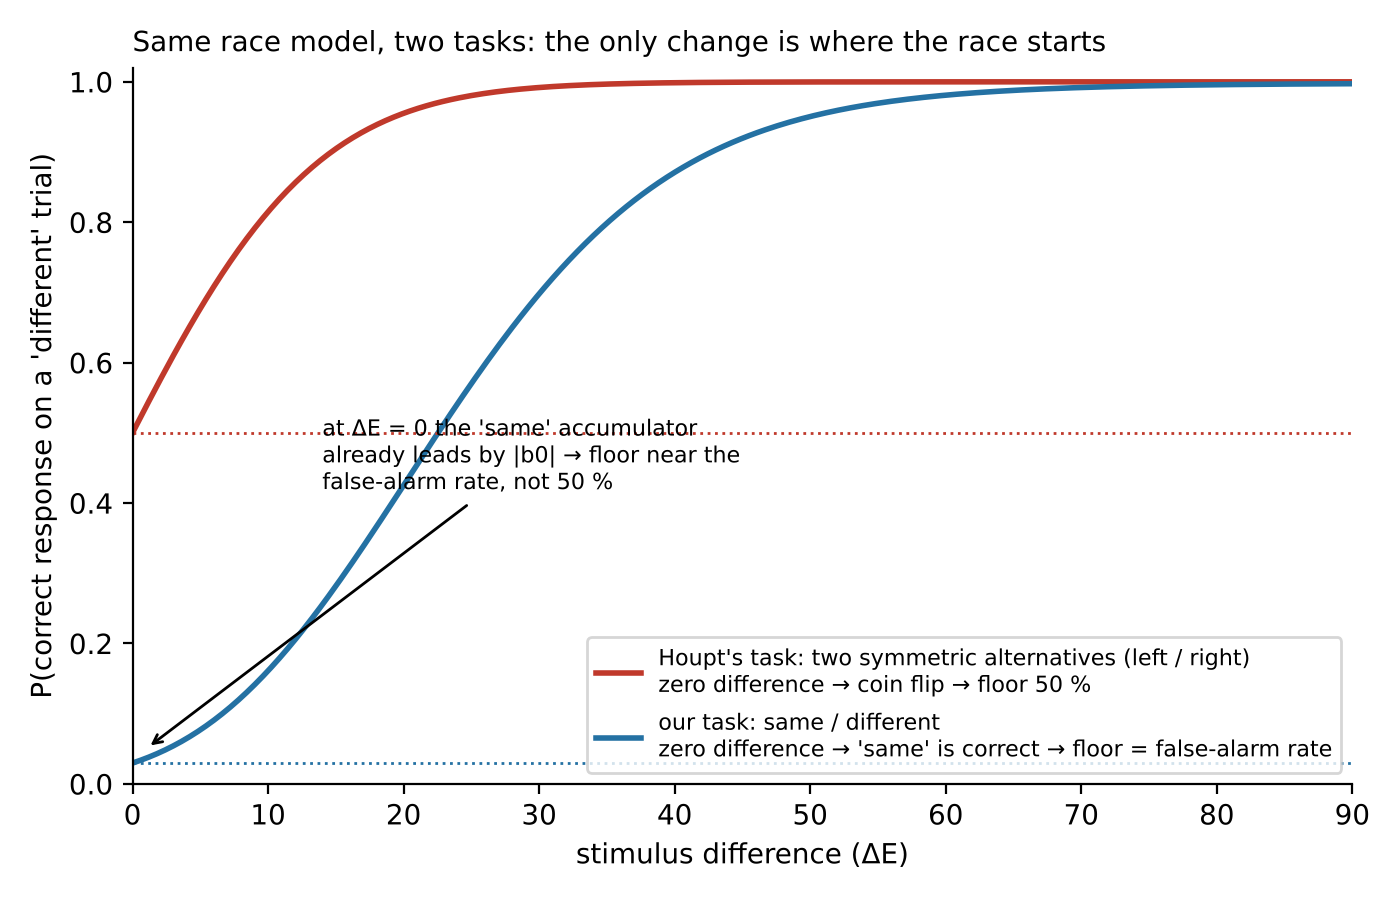
\includegraphics[width=\linewidth]{fig5_two_tasks}
\note{Illustrative curves with identical $\alpha$, $\alpha_2$ and $\sigma$; the blue curve adds a head start of the \emph{same} accumulator, $b_0 = -1.2$. The dotted lines mark the two floors.}
\end{figure}

\begin{figure}[htbp]
\caption{Posterior of $\alpha$ on EN01's Data With and Without the Criterion}
\label{fig:alphab0}
\centering
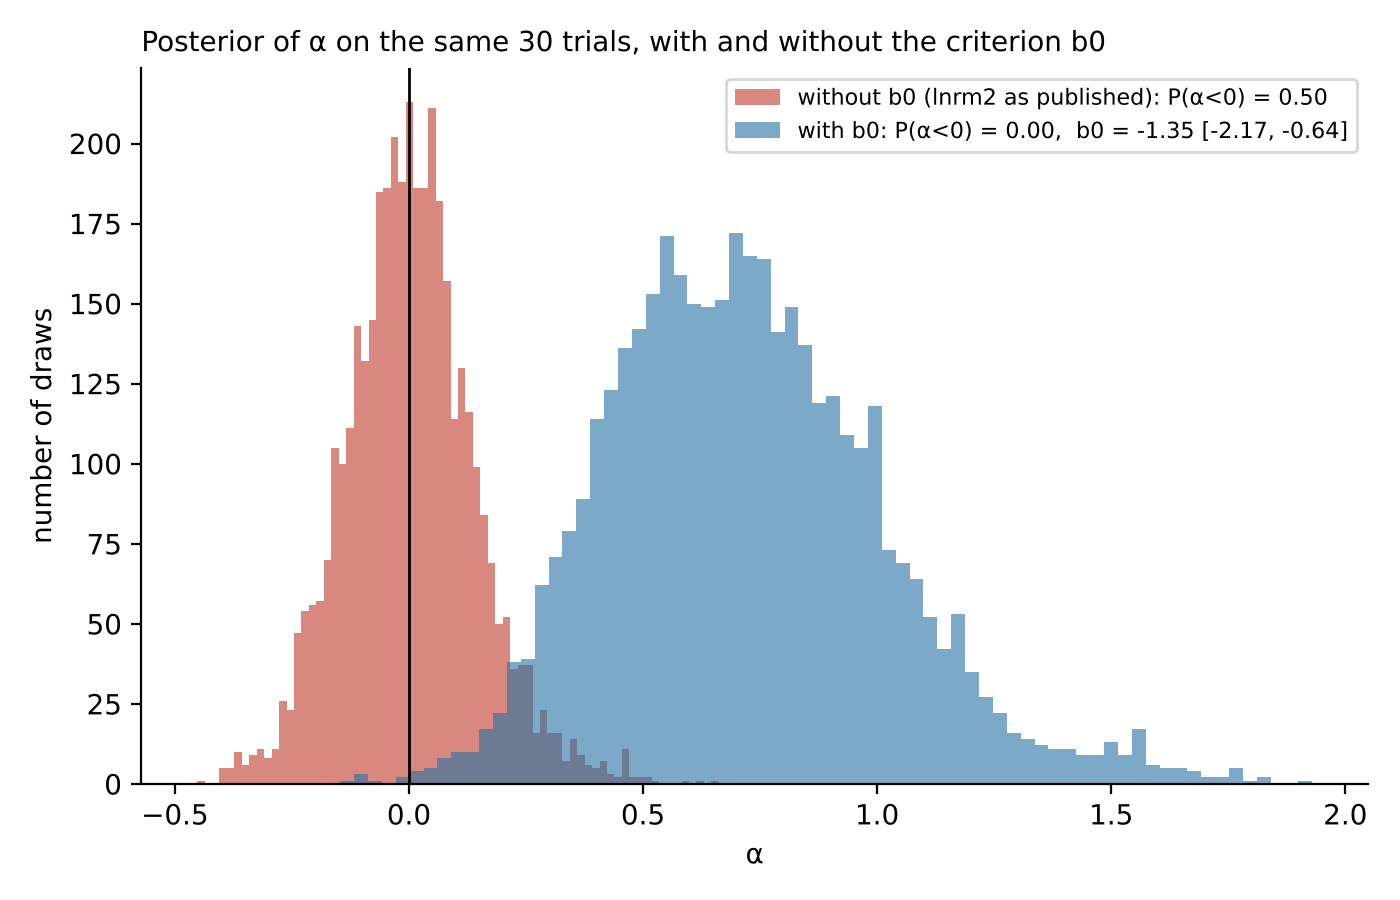
\includegraphics[width=\linewidth]{fig6_alpha_with_without_b0}
\end{figure}

\begin{figure}[htbp]
\caption{Posterior-Median Predictions With and Without the Criterion Against EN01's Data}
\label{fig:predb0}
\centering
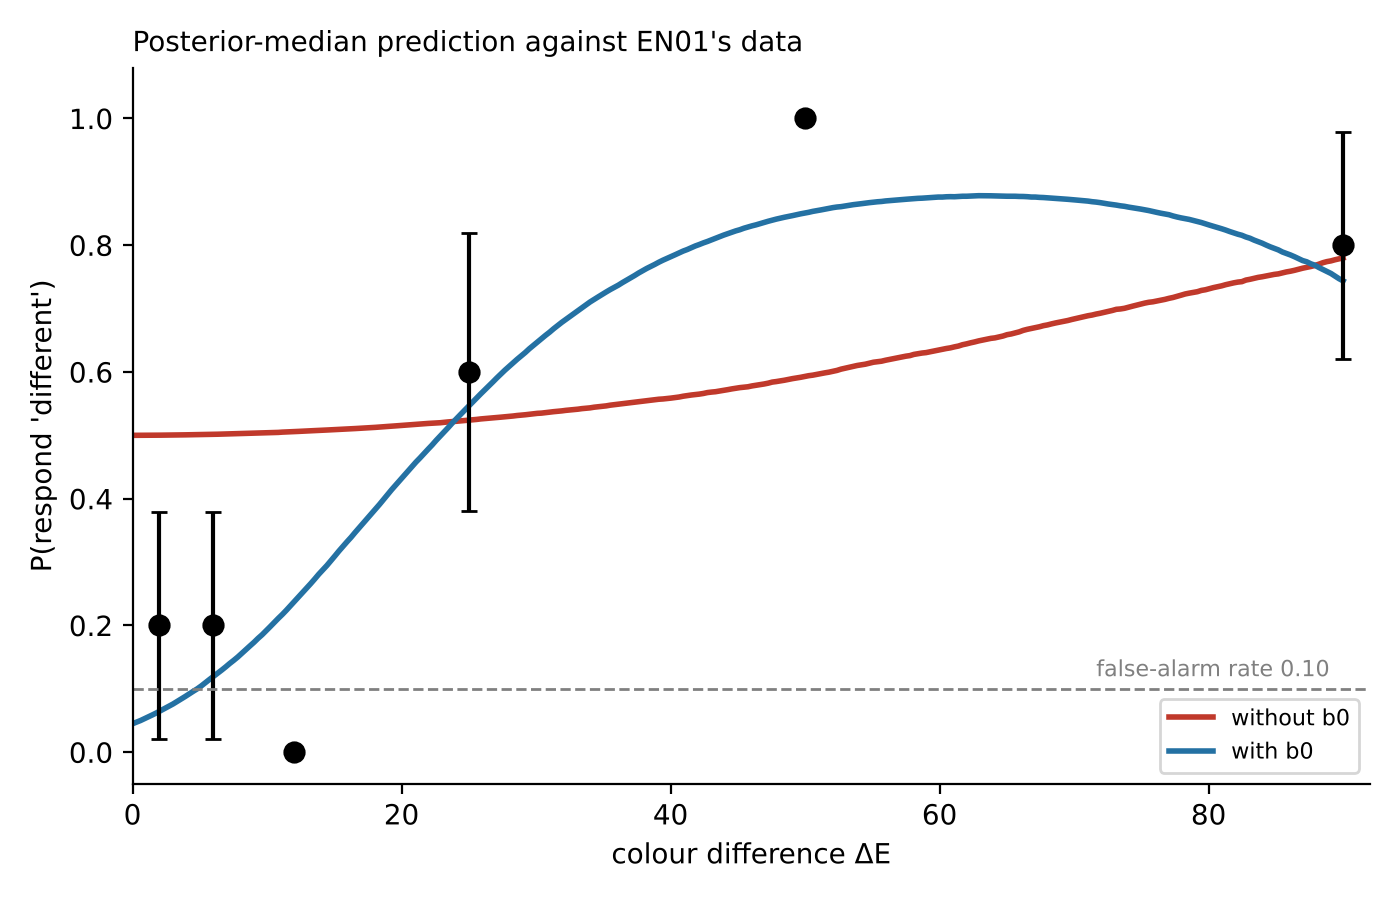
\includegraphics[width=\linewidth]{fig7_prediction_with_without_b0}
\note{The remaining underprediction at $\Delta E = 50$ (.85 predicted, 5/5 observed) reflects the shared $\sigma$ of accuracy and response time in the race model and is addressed in Section~\ref{sec:levels}.}
\end{figure}

\section{Revision 2: A Saturating Link Function}\label{sec:link}

The criterion fixes the floor; the quadratic term governs the top of the curve, and a quadratic with $\alpha_2 < 0$ has a single maximum beyond which it declines. On EN01's data the quadratic (with $b_0$) peaked at $\Delta E \approx 64$ and fell to $d_{\text{eff}} = 0.34$ at $\Delta E = 90$ (Figure~\ref{fig:links}), a shape forced by $-\alpha_2 x^2$ rather than by the data: the only observation above $\Delta E = 50$ is a single miss in five trials at 90, which the quadratic reads as an increase in difficulty and a saturating curve reads as a lapse (Figure~\ref{fig:linkpred}). We therefore adopted the authors' alternative link \citep[the \texttt{lnrm2a} model;][]{houpt2014}, $d(x) = \tfrac{1}{2} L \cdot \mathrm{logistic}\left(s\,(x - m)\right)$, with the ceiling $L$ estimated rather than fixed at 10, together with $b_0$. A linear link was also examined: it removed the sign ambiguity ($P(\alpha < 0) = .07$ without $b_0$) but cannot represent a steep rise followed by a plateau and placed the upper calibration point at $\Delta E = 78$--$95$, incompatible with the 5/5 performance of both recent pilots at $\Delta E = 25$--$50$. The two saturating shapes examined (logistic; saturating exponential) agreed on the \SI{50}{\percent} point (EN01: 25 vs 27; yyc1110: 16 vs 13) and differed on the plateau, for which the pilot design had no observations between $\Delta E = 28$ and 90 (Section~\ref{sec:levels}).

\begin{figure}[htbp]
\caption{Fitted Drift Advantage Under the Quadratic and the Logistic Link, Both With $b_0$}
\label{fig:links}
\centering
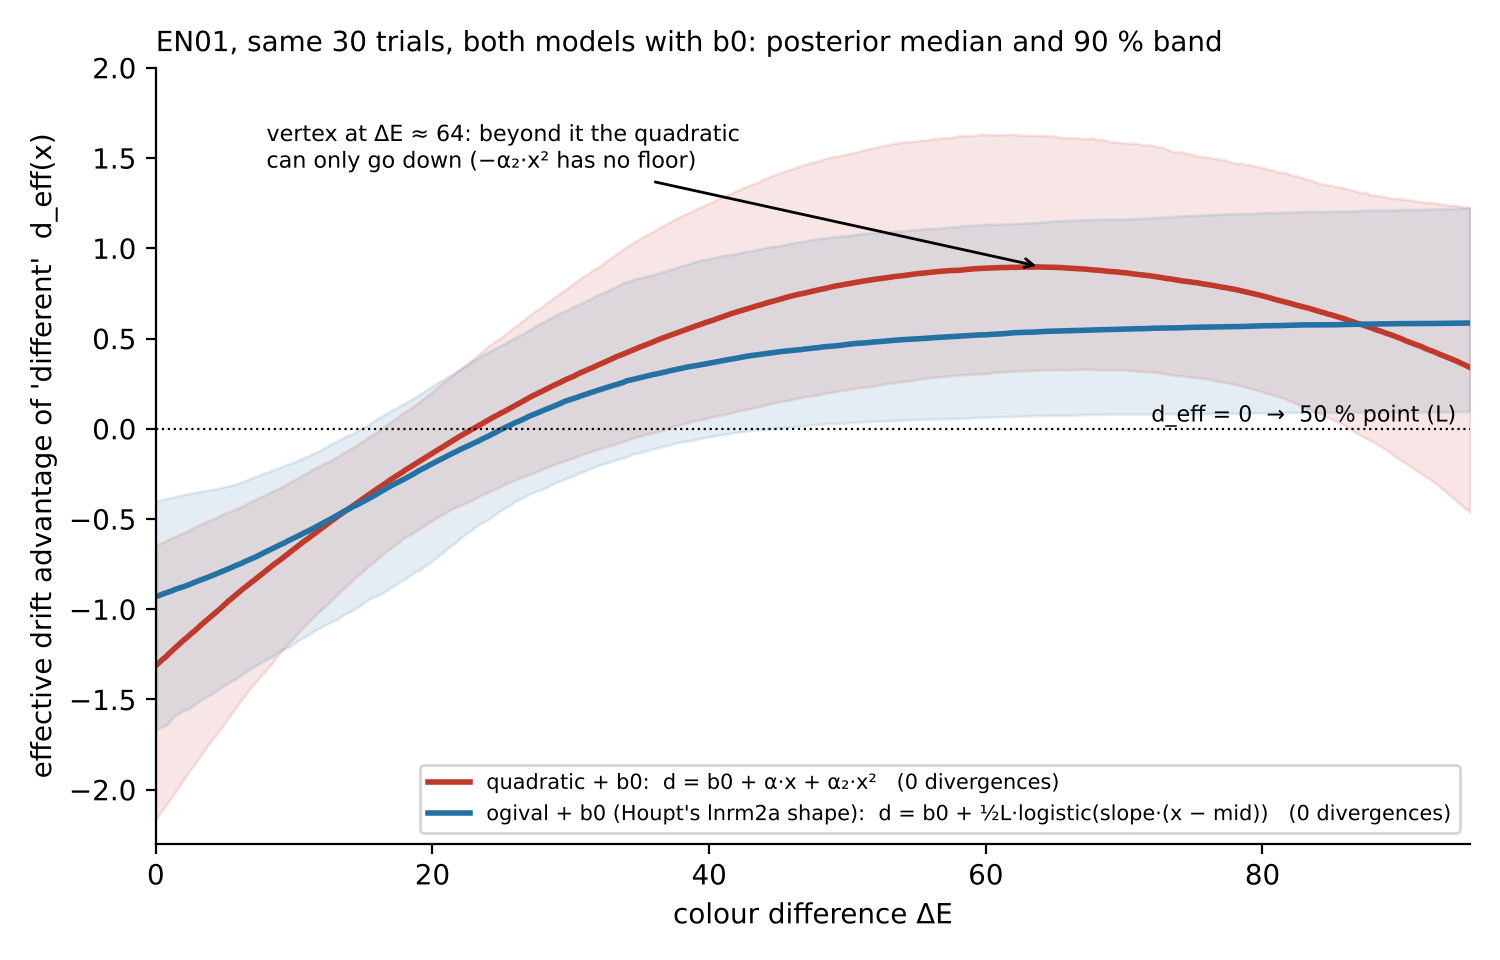
\includegraphics[width=\linewidth]{fig8_quadratic_vs_ogival_drift}
\note{Posterior medians with \SI{90}{\percent} bands; EN01, 30 trials. The quadratic's vertex is at $\Delta E \approx 64$.}
\end{figure}

\begin{figure}[htbp]
\caption{Predicted Proportion of \emph{Different} Responses Under the Two Links Against EN01's Data}
\label{fig:linkpred}
\centering
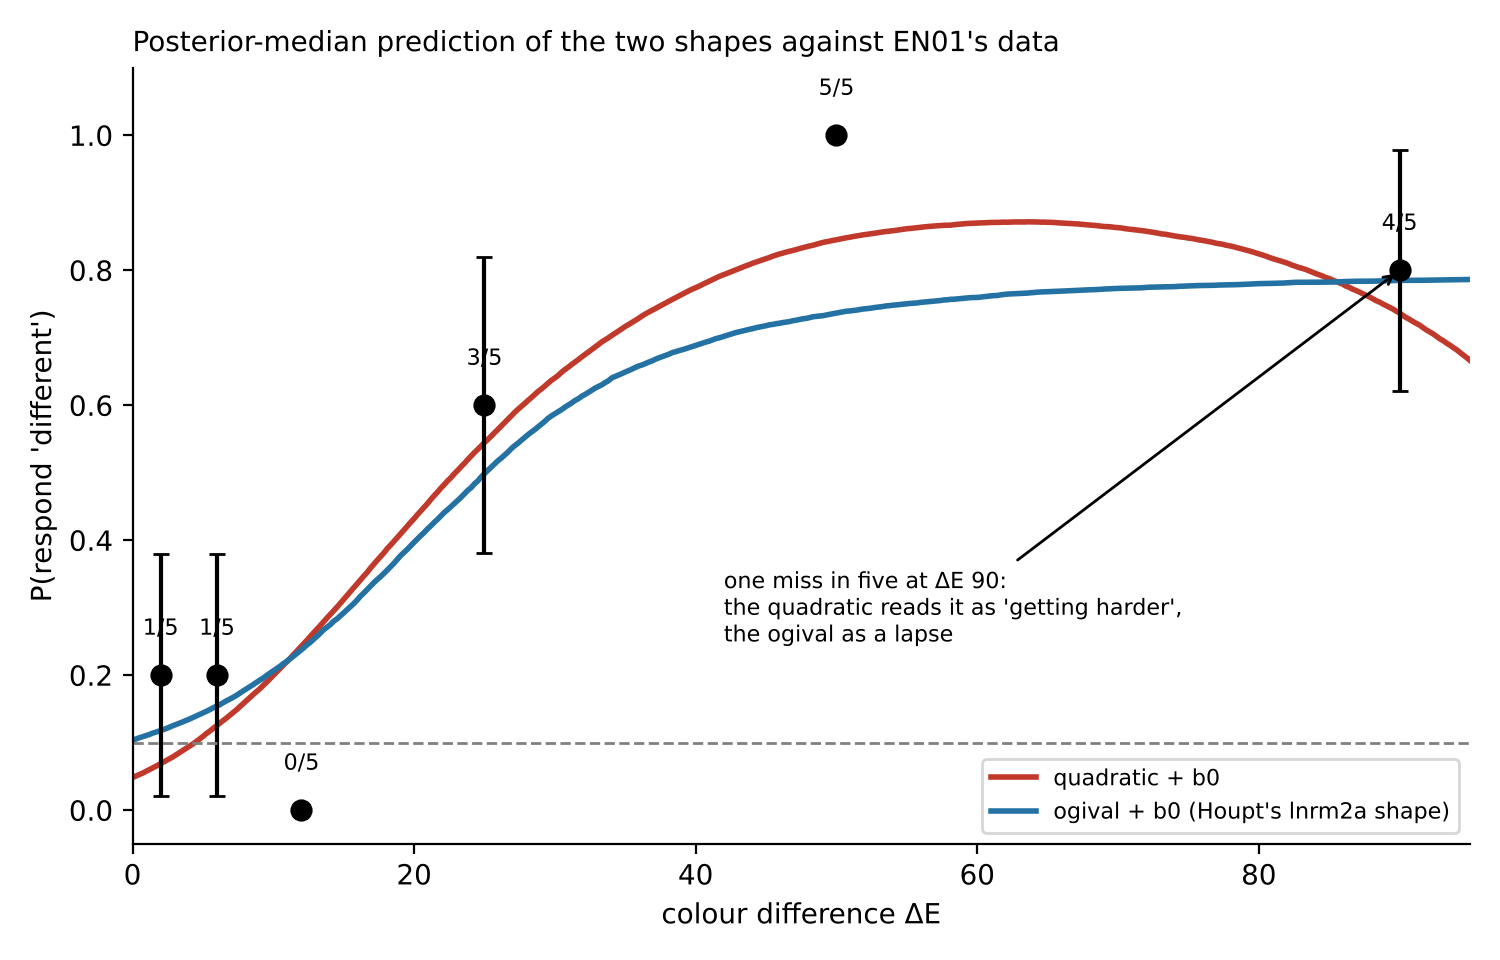
\includegraphics[width=\linewidth]{fig9_quadratic_vs_ogival_prediction}
\end{figure}

\section{Revision 3: Targets Defined as Psychometric Points, Estimated by the Posterior Median}\label{sec:estimator}

\paragraph{Targets.} The drift-separation targets 8.0 and 1.3 of \citet{houpt2014} were replaced by two points of the fitted function. L is the \SI{50}{\percent} point, the intensity at which $d_{\text{eff}}(x) = 0$, i.e.\ at which the stimulus-driven advantage exactly cancels the criterion. H is the plateau onset, the intensity at which the logistic reaches .9 of its ceiling, beyond which the model predicts no further speeding of responses. The \SI{50}{\percent} point depends neither on $\sigma$ nor on the shape of the upper curve and was stable across link functions. An accuracy-defined upper target (e.g.\ \SI{90}{\percent} correct) was rejected because in the race model accuracy and response-time dispersion share $\sigma$; with $\sigma \approx 1.0$--$1.2$, as observed under working-memory load, the model requires $d_{\text{eff}} \approx 1.1$ for \SI{90}{\percent} while the fitted ceilings were 0.6--0.9, so that the target was declared unreachable although participants were at 5/5. The plateau onset is read from the drift curve and is not subject to this coupling.

\paragraph{Estimator.} Both points are reported as the posterior median of their per-draw solutions rather than the mean used in the original R code. The per-draw solution is a ratio of posterior quantities whose denominator (the curvature or the slope) has mass near zero; such a distribution has no finite mean in practice. Figure~\ref{fig:seeds} shows the original model refitted to the same 30 trials with eight sampler seeds: the median of the inverted H lay between 422 and 492 in every run, whereas the mean ranged from $+486$ to $+764$ in six runs and was $-994$ and $-8{,}498$ in two, each flip produced by one or two negative draws. Figure~\ref{fig:mechanism} shows the mechanism: for $\alpha < 0$ a root exists only when $|\alpha_2| < \alpha^2/8$ and is then at least $80/|\alpha|$ $\Delta E$ in magnitude, diverging as $\alpha_2 \to 0$. Under the revised model (Figure~\ref{fig:newpoints}) the \SI{50}{\percent} point is compact (EN01: median 24.9, mean 26.2) and the plateau retains a right tail (median 36.3, mean 42.0, maximum 333), in the same direction as before, so the median is used for both.

\paragraph{Range handling.} If no \SI{50}{\percent} point exists (most draws have $b_0 \ge 0$, i.e.\ the observer responds \emph{different} at zero difference), L is set to the lowest level; if no plateau exists, H is set to the highest level; both are then clipped into the presentable range; and if $L \ge H$ after clipping, H is raised to the highest level. L is never lowered by this rule. Every step is recorded in the calibration file and shown to the experimenter.

\begin{figure}[htbp]
\caption{Mean and Median of the Inverted H Across Eight Sampler Seeds on the Same Data}
\label{fig:seeds}
\centering
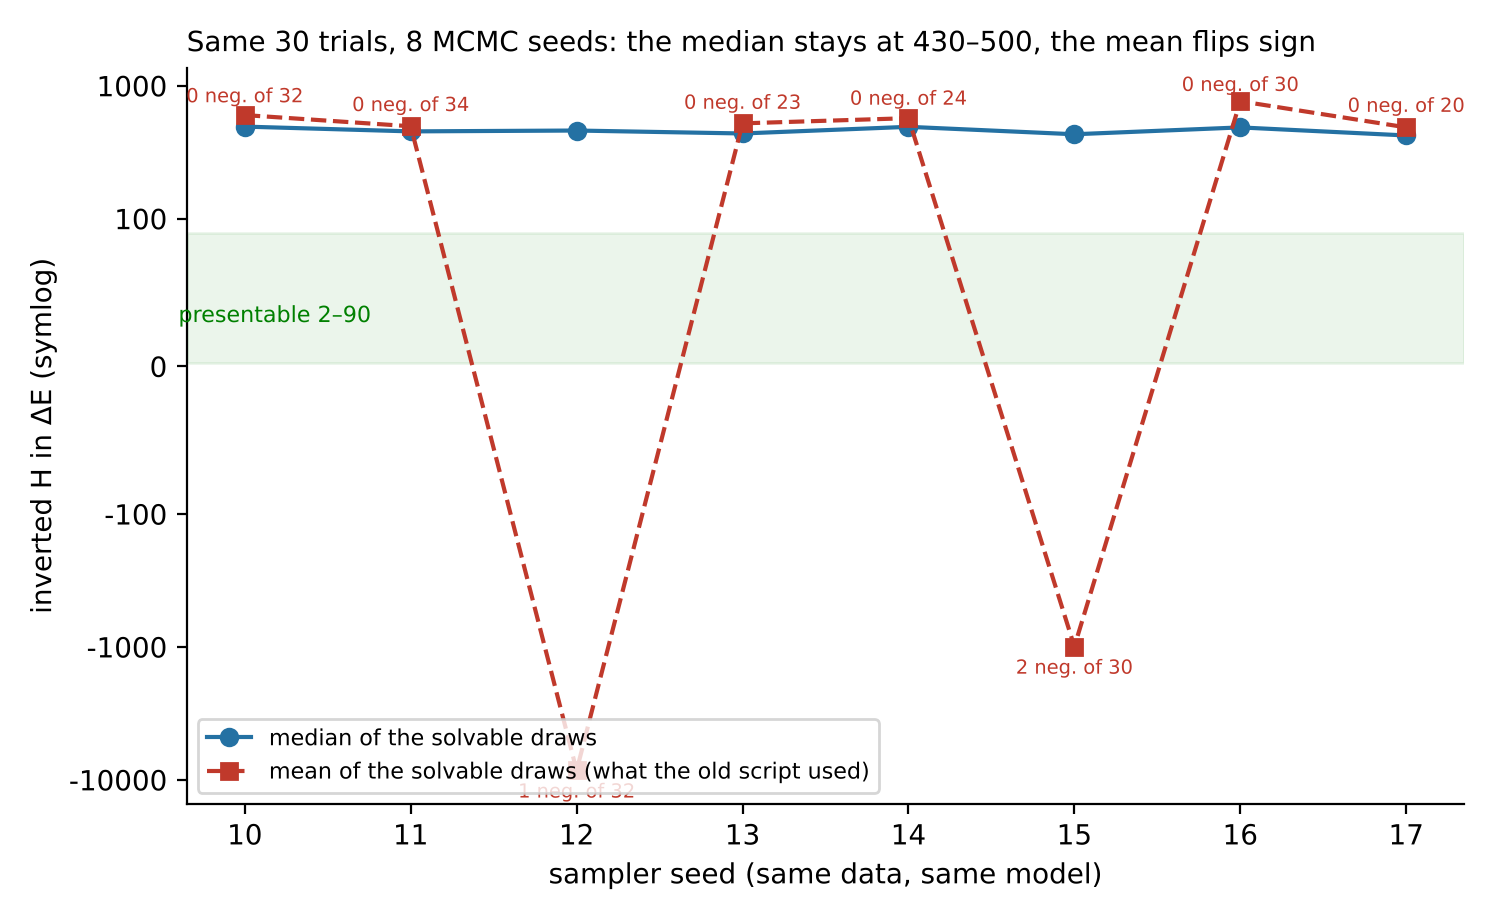
\includegraphics[width=\linewidth]{fig10_mean_vs_median_seeds}
\note{Original model (quadratic link, no criterion). Labels give the number of negative draws among the solvable draws for each seed.}
\end{figure}

\begin{figure}[htbp]
\caption{Inverted H as a Function of the Curvature Draw, for Three Values of the Slope}
\label{fig:mechanism}
\centering
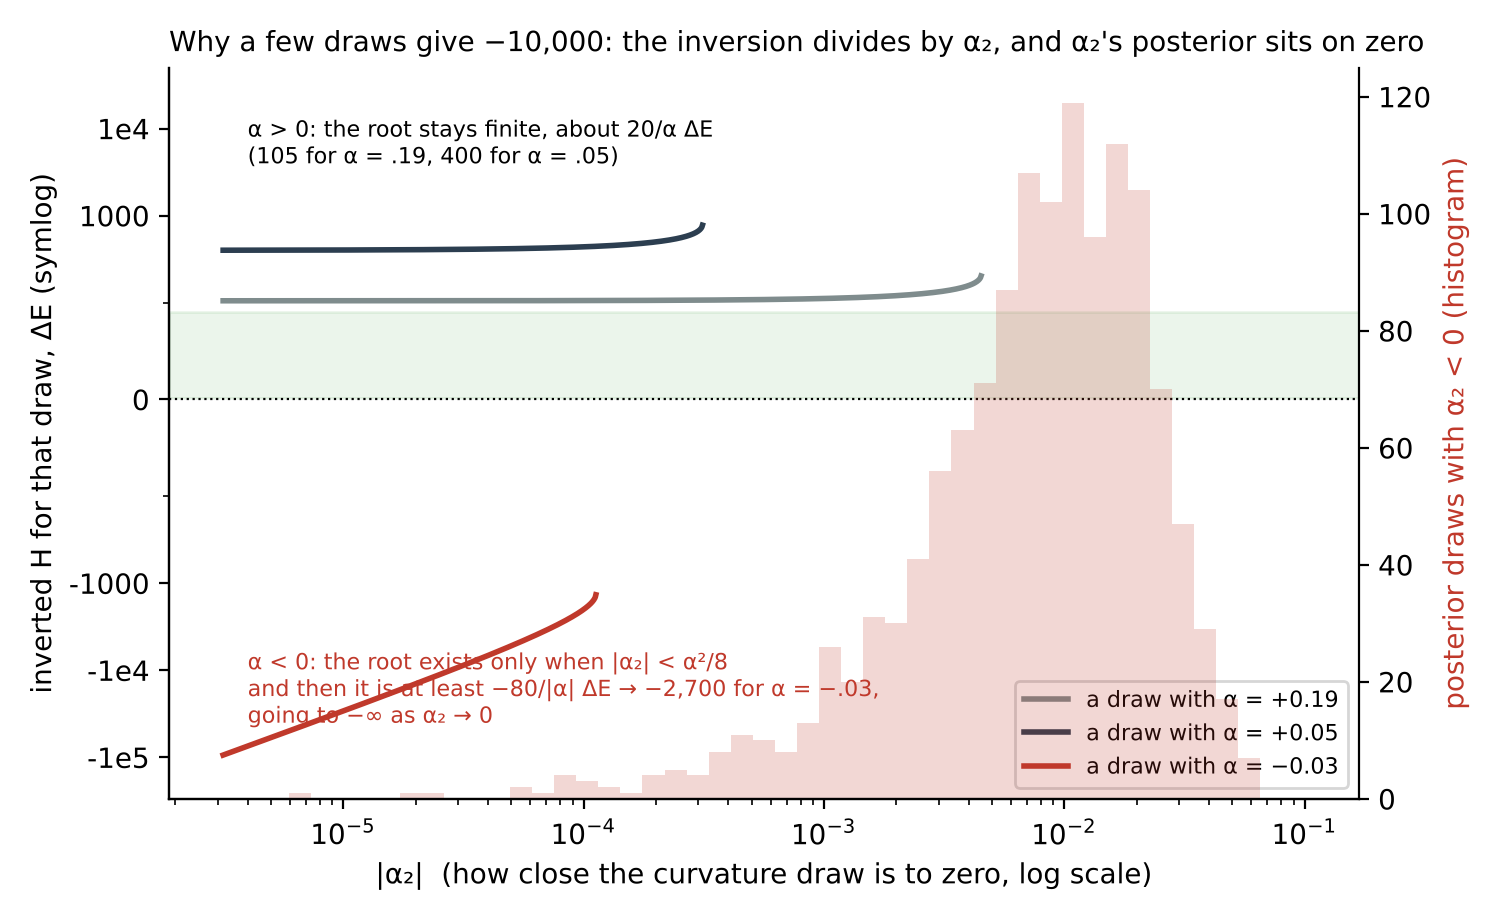
\includegraphics[width=\linewidth]{fig11_root_vs_alpha2}
\note{Symmetric-log ordinate; the histogram is the posterior of $\alpha_2$ for the draws with $\alpha_2 < 0$. Positive-slope draws give bounded roots (about $20/\alpha$ $\Delta E$); negative-slope draws give roots that diverge as $\alpha_2 \to 0$.}
\end{figure}

\begin{figure}[htbp]
\caption{Posterior Draws of the Two Calibration Points Under the Revised Model (Logistic Link With $b_0$), EN01}
\label{fig:newpoints}
\centering
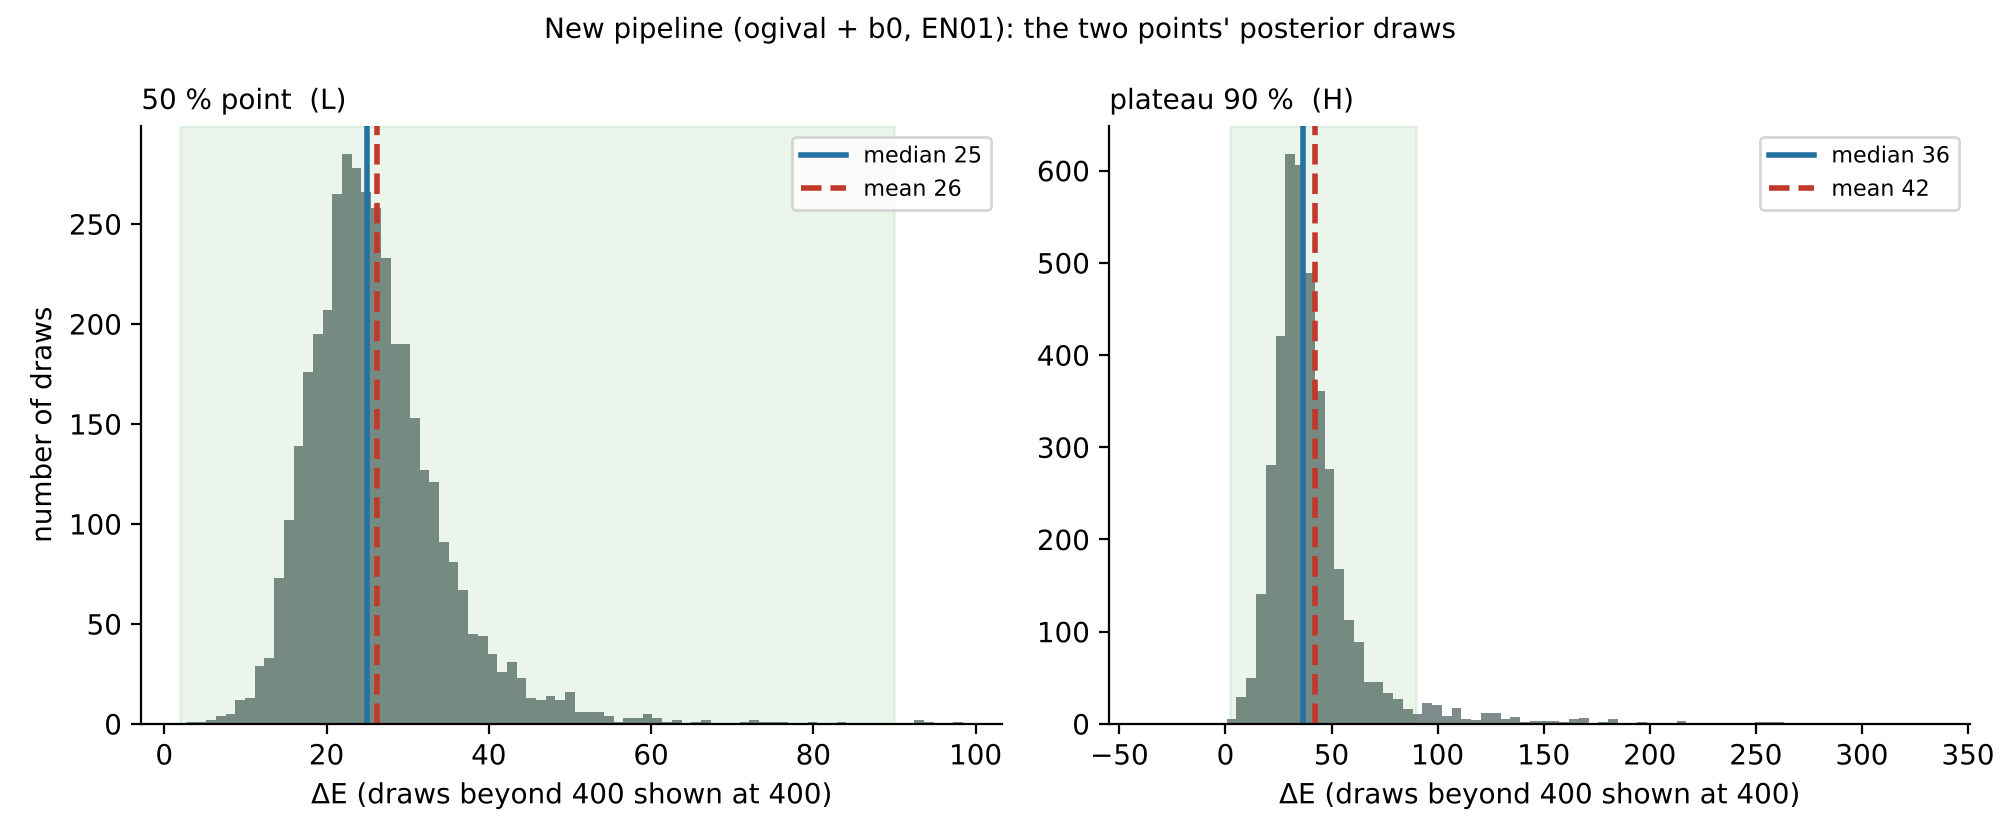
\includegraphics[width=\linewidth]{fig12_new_pipeline_points}
\note{Left: \SI{50}{\percent} point; right: plateau onset. Draws beyond 400 $\Delta E$ are shown at 400.}
\end{figure}

\section{Revision 4: Stimulus Levels}\label{sec:levels}

The colour levels were revised in two steps (Table~\ref{tab:levels}). First, the levels 2, 6 and 12, at which all three pilots were at the false-alarm floor (Table~\ref{tab:colour}; Figure~\ref{fig:pilots}), were moved onto the rising part of the function, between 12 and 30. Second, because H is now read from the plateau onset, the two upper levels were placed at 45 and 70, on the bend of the fitted curves, where the pilot design had no observations (Figure~\ref{fig:plateauci}); the level 90 had only confirmed a ceiling already established at 50. The number of levels (six) and trials per level (five) were kept, so that the session length is unchanged. A simulation of an EN01-like observer (Figure~\ref{fig:levelsim}) indicates that, at five trials per level, the three level sets yield similar uncertainty in the plateau estimate (mean \SI{90}{\percent} interval width 79, 103 and 94 $\Delta E$; median absolute error 11, 10.5 and 9.7 $\Delta E$) and in the \SI{50}{\percent} point (error 5--6 $\Delta E$); the revision is therefore justified by coverage of the estimated quantity, not by a demonstrated gain in precision, which would require more trials in the 30--70 range. A participant whose plateau lies above 70 will have H clipped to 70 and flagged.

Refitting the two recent pilots with the revised model and rules gave colour $L = 25.2$ ($[14.8, 42.1]$) and $H = 36.0$ ($[18.3, 80.8]$) for EN01 and $L = 15.2$ ($[8.6, 21.2]$) and $H = 26.9$ ($[18.2, 47.6]$) for yyc1110, both within range, with 0--2 divergent transitions.

\begin{table}[htbp]
\caption{Colour Calibration Levels ($\Delta E_{00}$) Before and After the Revisions}
\label{tab:levels}
\small
\setlength{\tabcolsep}{4pt}
\begin{tabular}{@{}llccc@{}}
\toprule
Level set & Levels & Floor & Slope (12--30) & Bend / ceiling \\
\midrule
Pilot design     & 2, 6, 12, 25, 50, 90  & 2, 6, 12   & 25         & --- / 50, 90 \\
Revision, step 1 & 8, 14, 20, 28, 40, 90 & 8 (partly) & 14, 20, 28 & 40 / 90 \\
Revision, step 2 & 8, 14, 20, 28, 45, 70 & 8 (partly) & 14, 20, 28 & 45 / 70 \\
\bottomrule
\end{tabular}
\normalsize
\note{Regions are defined from the three pilots' data (Figure~\ref{fig:pilots}). Five trials per level in all sets.}
\end{table}

\begin{figure}[htbp]
\caption{Colour Calibration Performance of the Three Pilots and the Three Level Sets}
\label{fig:pilots}
\centering
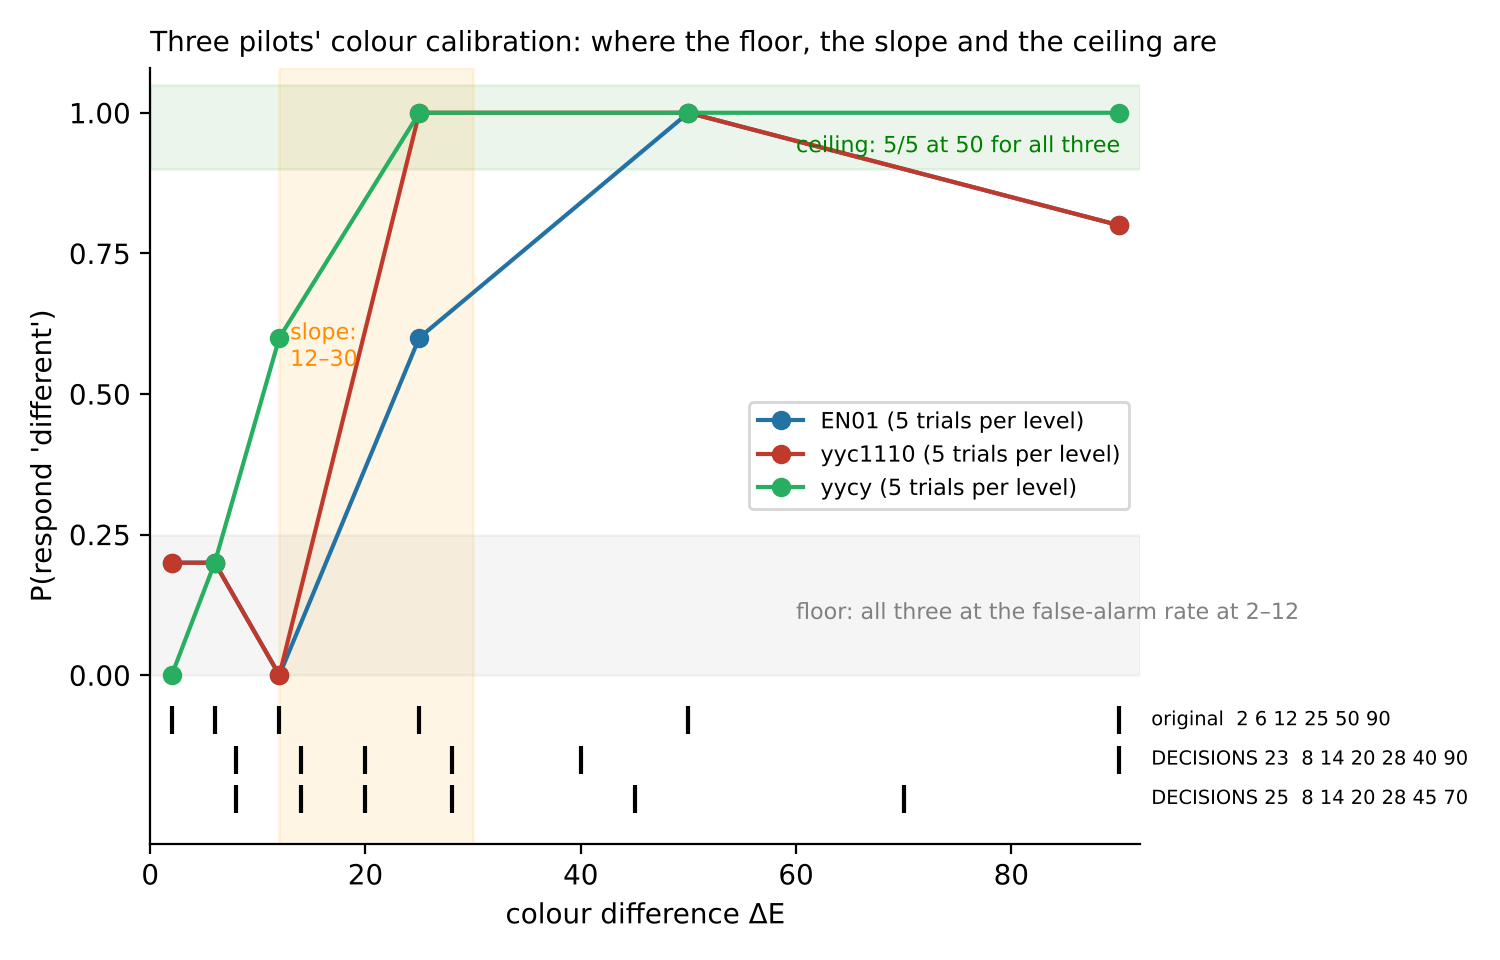
\includegraphics[width=\linewidth]{fig13_pilots_levels}
\end{figure}

\begin{figure}[htbp]
\caption{Fitted Drift Curves, Plateau Estimates, and the Old and New Upper Levels}
\label{fig:plateauci}
\centering
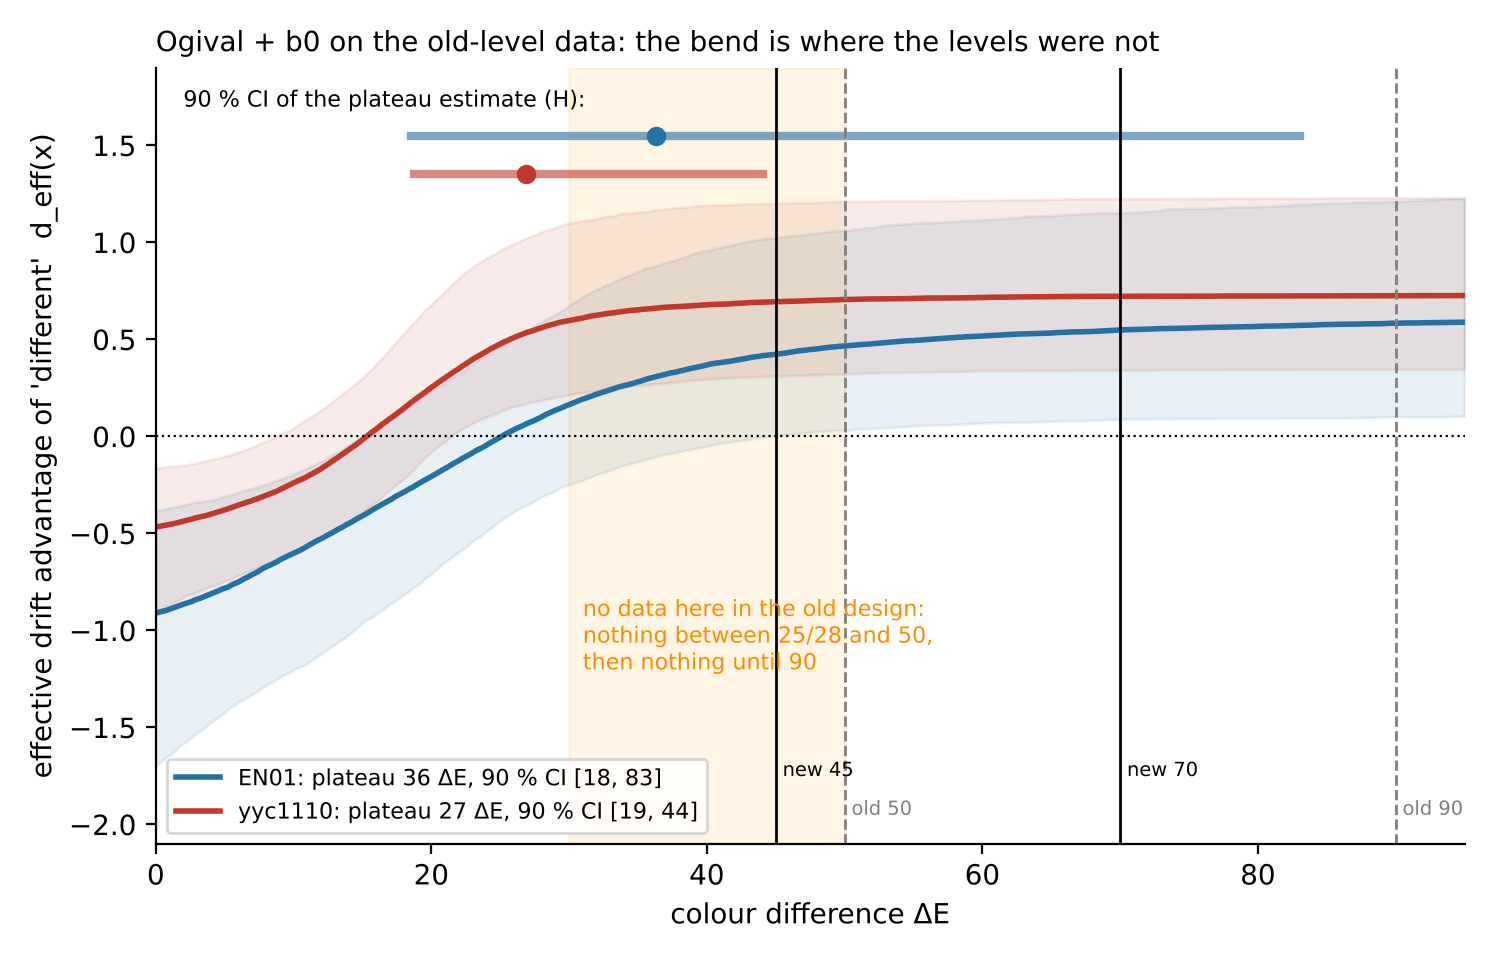
\includegraphics[width=\linewidth]{fig14_plateau_ci_levels}
\note{Logistic link with $b_0$, EN01 and yyc1110; horizontal bars are \SI{90}{\percent} intervals of the plateau onset. The shaded region (30--50) is where both curves bend and where the pilot design had no trials.}
\end{figure}

\begin{figure}[htbp]
\caption{Simulated Uncertainty of the Plateau Estimate Under the Three Level Sets}
\label{fig:levelsim}
\centering
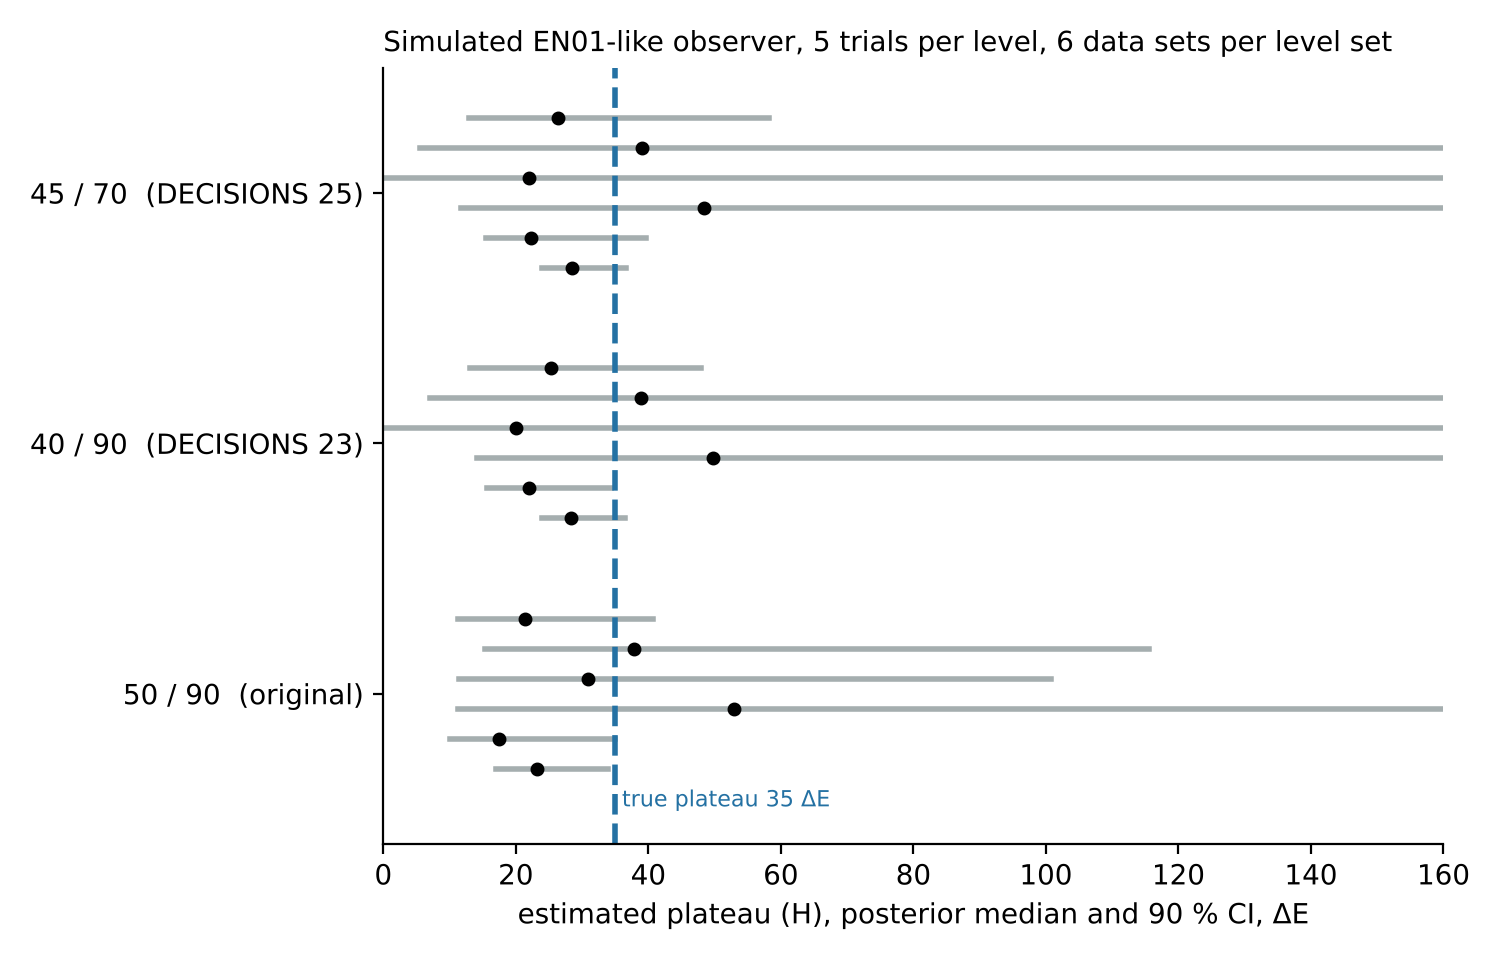
\includegraphics[width=\linewidth]{fig15_plateau_ci_by_levelset}
\note{Observer parameters taken from EN01's fit (true plateau 35 $\Delta E$); five trials per level; six simulated data sets per level set.}
\end{figure}

\section{The Auditory Dimension}\label{sec:sound}

\paragraph{Selective-influence check.} EN01's main task (576 trials) allowed a check of whether the auditory H/L manipulation satisfied the ordering of survivor functions required for the survivor interaction contrast \citep{houpttownsend2010}. Because the colour levels were identical in that session, the double-change cells were pooled by sound level (HH + HL vs.\ LH + LL). The survivor functions of correct response times crossed and did not separate (Figure~\ref{fig:survivor}): one-sided Kolmogorov--Smirnov tests gave $p = .55$ in the predicted direction and $p = .39$ in the violating direction; the single-channel cells HA vs.\ LA gave $p = .46$; all eight dominance tests of \citet{houpt2014} had $p$ between .20 and .94; accuracy was .92 (H) vs.\ .90 (L) and median response time 0.73 vs.\ 0.74 s. The auditory manipulation was therefore ineffective for this participant.

\paragraph{Cause.} The consonant-pair scale contains almost no sufficiently confusable pairs: 14 of the 240 ordered pairs have $d' < 0.8$, and six consonants (b, m, n, s, and the two postalveolar fricatives sh and zh) have no foil below $d' = 1.0$. Both recent pilots were at ceiling at all but one sound level in calibration (Figure~\ref{fig:dscale}), and the revised model placed their \SI{50}{\percent} points below zero ($-1.2$ and $-0.8$), i.e.\ below the lowest presentable level; L was set to the lowest level and flagged in both cases. The rising part of the psychometric function lies to the left of the scale.

\paragraph{Decision.} Rather than restrict L to the few available pairs, which would confound level with articulatory feature \citep[place pairs only; cf.][]{millernicely1955}, the consonants will be presented in speech-shaped noise at one signal-to-noise ratio held constant for the whole session. Noise compresses the distinctiveness of every pair towards zero and thereby extends the scale at its lower end; it is the manipulation under which the \citet{millernicely1955} matrices, from which the scale is derived, were obtained (Figure~\ref{fig:snr}). The SNR is a session constant, not a factor: H and L continue to differ only by consonant pair. The mixing module built for the companion GRT experiment was adapted: exact SNR relative to the active portion of each token, long-term-average-spectrum-shaped noise pooled over the 192 tokens, fixed output level, and a deterministic noise seed per presentation, $\text{seed} = h(\text{phase}, \text{trial}, \text{slot})$, identical across participants (a fixed stimulus set) and different for the studied item and the probe, so that a \emph{same} probe is the same consonant in a different noise sample and cannot be matched on the noise waveform. Seeds and SNR are written to every data row and the presented waveform can be rebuilt bit-for-bit.

\paragraph{SNR pilot (preliminary).} The SNR is being chosen with the pure-perception consonant test (two syllables, same/different, 108 trials, feedback) at 0, $+6$ and $+12$ dB. The first listener (yyc1116, a non-native listener) gave, at 0 dB, a false-alarm rate of .47 and hit rates of .50--.90 across the six levels ($d' = 0.07$--$1.35$), i.e.\ performance near chance except at the easiest level; at $+12$ dB, a false-alarm rate of .23 and hit rates of .58--.92. Two observations follow. First, speech-shaped noise is a more effective masker than the flat-spectrum noise of \citet{millernicely1955}, so the nominal SNR of their matrices does not transfer; the per-SNR scale will be taken from the matrix whose overall performance matches the pilot, not from the matrix with the same nominal SNR. Second, the drop in false alarms from .47 to .23 with increasing SNR suggests that part of the \emph{different} responses at low SNR reflected the audible difference between noise samples; this will be examined in the trial-level data and, if confirmed, addressed in the instructions. Native listeners are expected to tolerate a lower SNR \citep{cutler2004}; the final value will be set from pilots drawn from the intended participant population. The $+6$ dB condition and the trial-level analysis were pending at the time of writing.

\begin{figure}[htbp]
\caption{Survivor Functions of Correct Response Times by Auditory Level in EN01's Main Task}
\label{fig:survivor}
\centering
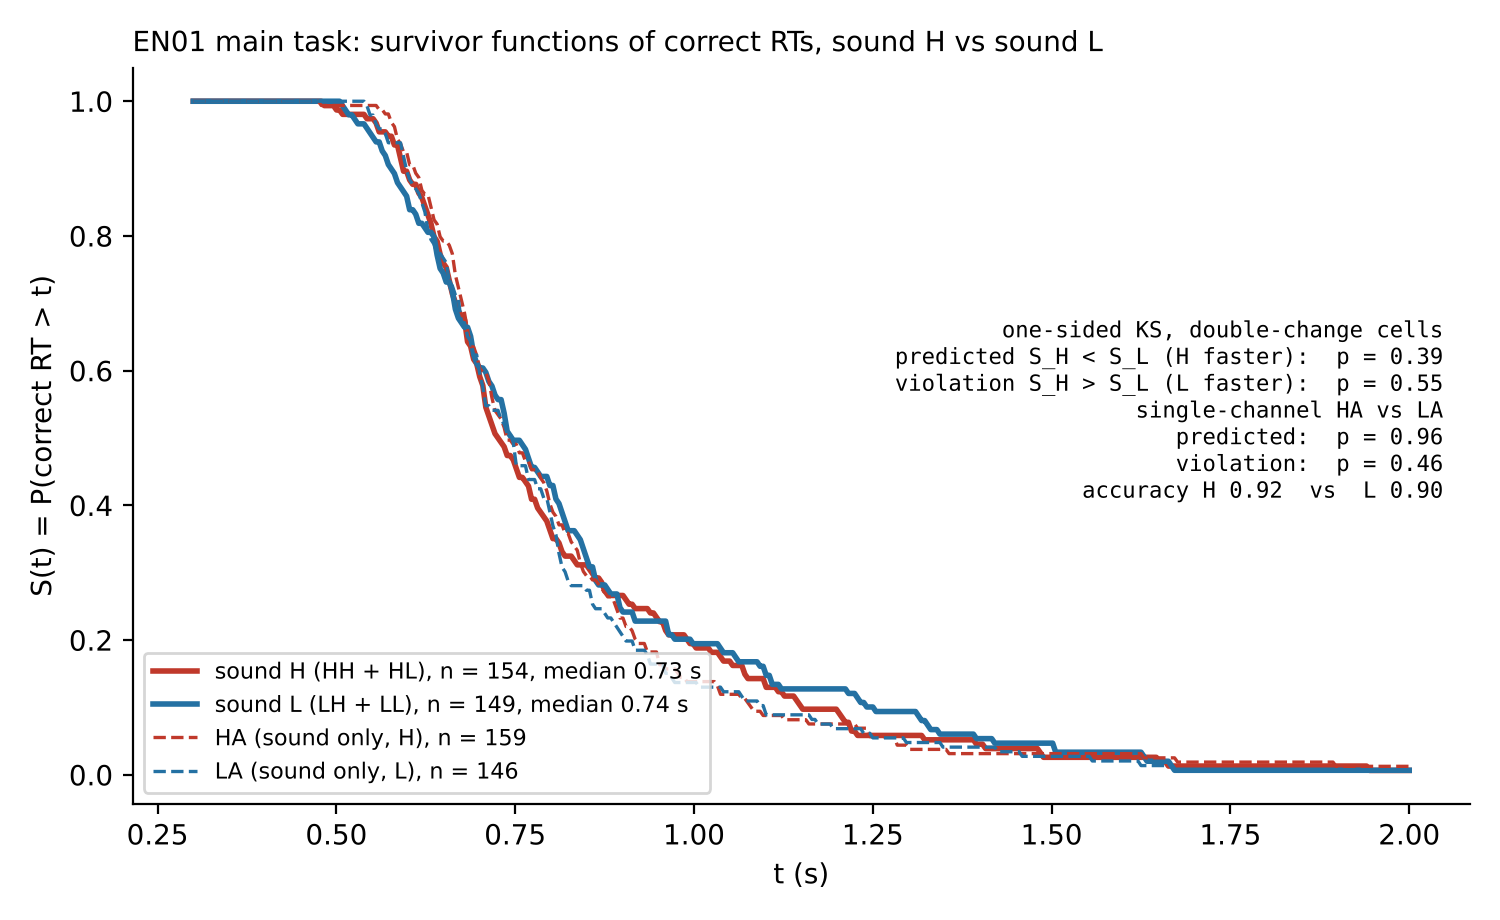
\includegraphics[width=\linewidth]{fig16_sound_survivor_functions}
\note{Solid: double-change cells pooled by sound level; dashed: single-channel cells HA vs.\ LA. One-sided Kolmogorov--Smirnov $p$ values in the legend.}
\end{figure}

\begin{figure}[htbp]
\caption{The Consonant-Pair $d'$ Scale and EN01's Auditory Calibration}
\label{fig:dscale}
\centering
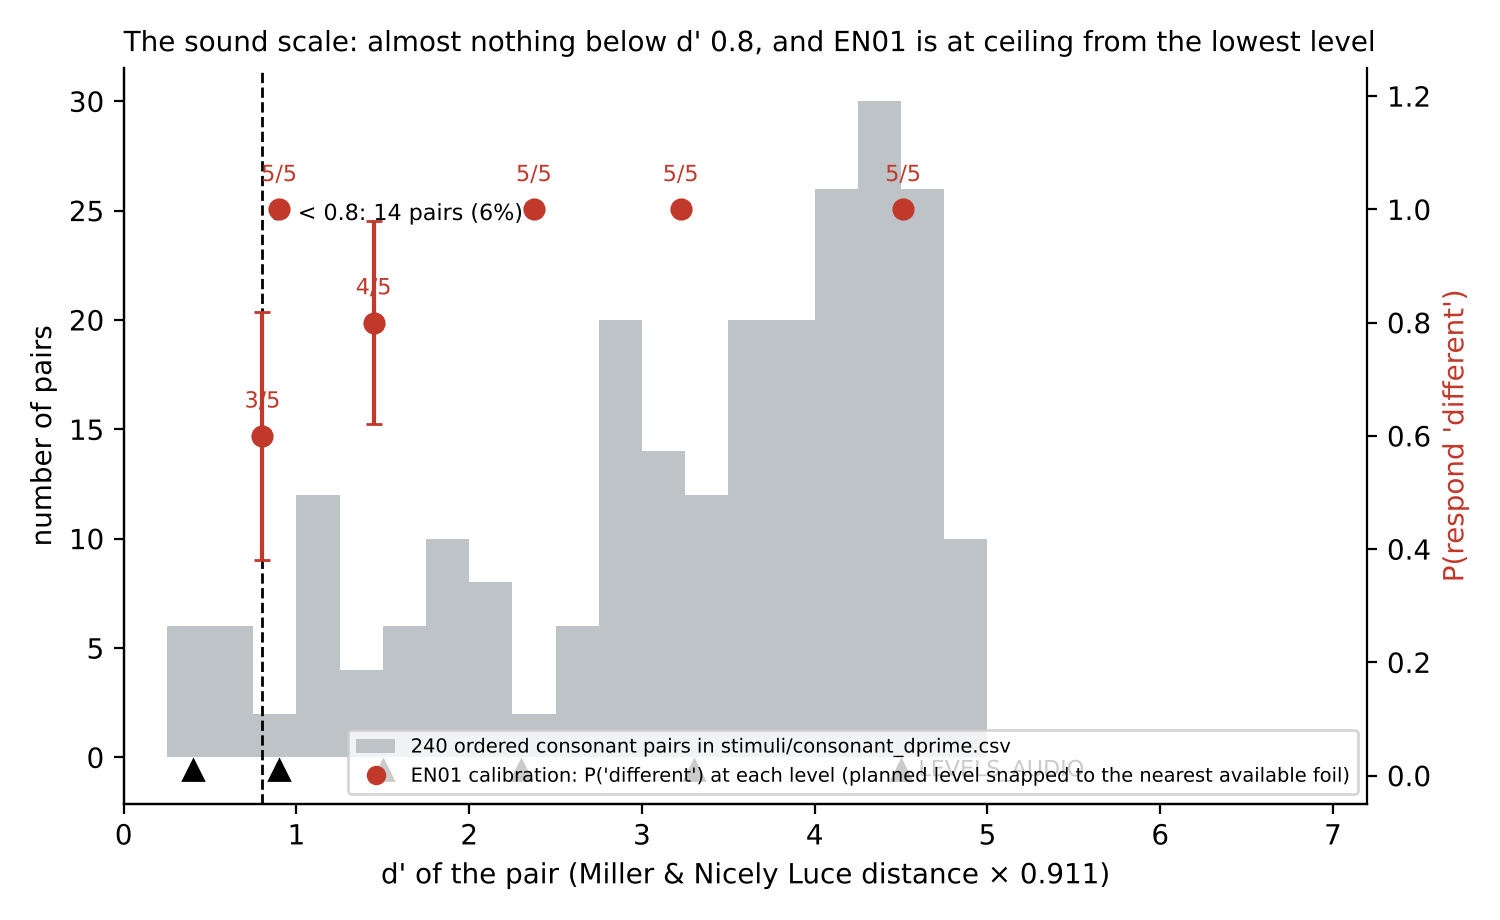
\includegraphics[width=\linewidth]{fig17_dprime_scale_vs_EN01}
\note{Histogram: the 240 ordered pairs of the scale; the vertical line marks $d' = 0.8$. Points: proportion of \emph{different} responses at each calibration level (actual $d'$ after snapping to available foils).}
\end{figure}

\begin{figure}[htbp]
\caption{Compression of the Pair Scale With Decreasing Signal-to-Noise Ratio in the Miller and Nicely (1955) Data}
\label{fig:snr}
\centering
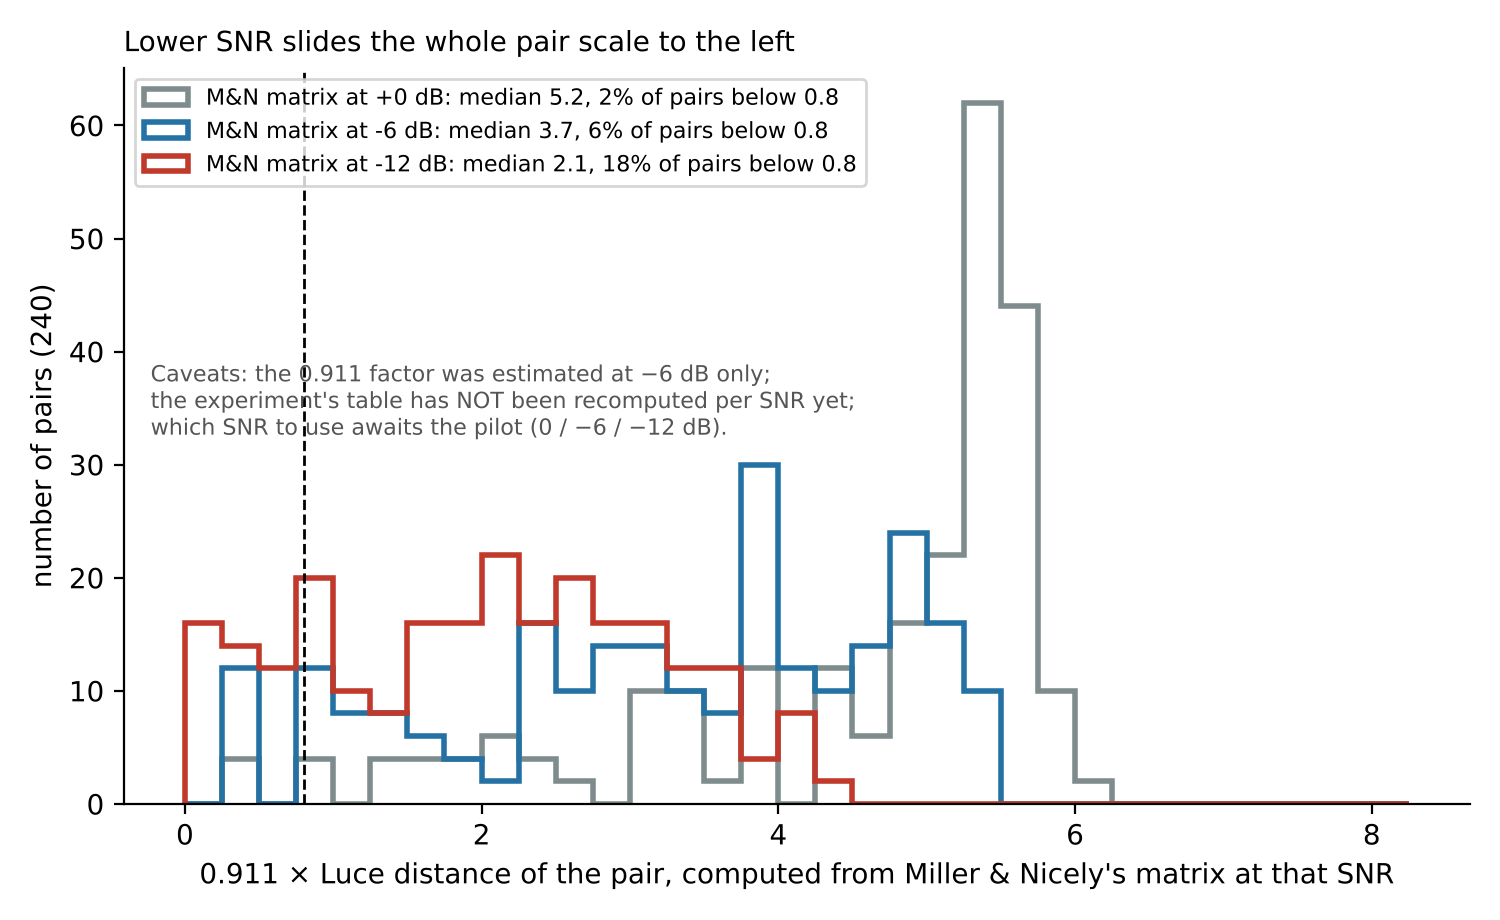
\includegraphics[width=\linewidth]{fig18_snr_shifts_scale}
\note{$d' = 0.911 \times$ Luce distance \citep{luce1963} computed from the confusion matrices at 0, $-6$ and $-12$ dB. The factor 0.911 was estimated at $-6$ dB only; the table used in the experiment has not yet been recomputed per SNR, and the SNR itself awaits the pilot.}
\end{figure}

\section{Summary of Revisions}

\begin{enumerate}
\item Race model: an intercept $b_0$ (same/different criterion) added to the drift advantage; $b_0 = 0$ recovers the published model.
\item Link: the logistic (\texttt{lnrm2a}) form with estimated ceiling replaces the quadratic.
\item Targets: L is the \SI{50}{\percent} point, H the plateau onset; both estimated by the posterior median; out-of-range handling never lowers L.
\item Colour levels: $\{8, 14, 20, 28, 45, 70\}$ $\Delta E_{00}$, six levels, five trials each.
\item Auditory stimuli: all consonants presented in speech-shaped noise at one session-wide SNR, with deterministic per-presentation seeds; SNR to be fixed by the pure-perception pilot.
\end{enumerate}

\begin{thebibliography}{}

\bibitem[Cutler et al.(2004)Cutler, Weber, Smits, and Cooper]{cutler2004}
Cutler, A., Weber, A., Smits, R., \& Cooper, N. (2004). Patterns of English phoneme confusions by native and non-native listeners. \emph{Journal of the Acoustical Society of America, 116}(6), 3668--3678. \url{https://doi.org/10.1121/1.1810292}

\bibitem[Houpt et al.(2014)Houpt, Blaha, McIntire, Havig, and Townsend]{houpt2014}
Houpt, J. W., Blaha, L. M., McIntire, J. P., Havig, P. R., \& Townsend, J. T. (2014). Systems factorial technology with R. \emph{Behavior Research Methods, 46}(2), 307--330. \url{https://doi.org/10.3758/s13428-013-0377-3}

\bibitem[Houpt and Townsend(2010)]{houpttownsend2010}
Houpt, J. W., \& Townsend, J. T. (2010). The statistical properties of the survivor interaction contrast. \emph{Journal of Mathematical Psychology, 54}(5), 446--453. \url{https://doi.org/10.1016/j.jmp.2010.06.006}

\bibitem[Kontsevich and Tyler(1999)]{kontsevich1999}
Kontsevich, L. L., \& Tyler, C. W. (1999). Bayesian adaptive estimation of psychometric slope and threshold. \emph{Vision Research, 39}(16), 2729--2737. \url{https://doi.org/10.1016/S0042-6989(98)00285-5}

\bibitem[Luce(1963)]{luce1963}
Luce, R. D. (1963). Detection and recognition. In R. D. Luce, R. R. Bush, \& E. Galanter (Eds.), \emph{Handbook of mathematical psychology} (Vol. 1, pp. 103--189). Wiley.

\bibitem[Macmillan and Creelman(2005)]{macmillan2005}
Macmillan, N. A., \& Creelman, C. D. (2005). \emph{Detection theory: A user's guide} (2nd ed.). Lawrence Erlbaum.

\bibitem[Miller and Nicely(1955)]{millernicely1955}
Miller, G. A., \& Nicely, P. E. (1955). An analysis of perceptual confusions among some English consonants. \emph{Journal of the Acoustical Society of America, 27}(2), 338--352. \url{https://doi.org/10.1121/1.1907526}

\end{thebibliography}

\end{document}
